\section{Background}\label{sec:background}

\subsection{Unemployment}

A program that automatically generates job applications would obviously be of
most use to people actively searching for a job. These people might currently
hold a job while looking for better opportunities. However it is reasonable to
assume that a significant number of them are unemployed, and thus it seems
pertinent to have a closer look at unemployment.

There are different types of unemployment, and the effect of applying for jobs
better and faster through automatic generation of the application will vary
greatly among them.
If there is a mismatch between offered and demanded skills, called structural
unemployment, little can be done through writing of job applications to fill
these jobs.%(https://en.wikipedia.org/wiki/Structural_unemployment)
Likewise if there is a downturn in the economy and no jobs are available for the
unemployed to apply for -- this is called cyclical unemployment.
%(https://en.wikipedia.org/wiki/Unemployment#Cyclical_unemployment)
The third broad category of unemployment is frictional unemployment, which
constitutes time spent between jobs on searching or transferring from one job to
another.%(https://en.wikipedia.org/wiki/Frictional_unemployment)
For this type of unemployment a more effective method of applying for jobs could
potentially shorten the unemployment period greatly. The same holds true
whenever there is an upturn in the economy and the cyclical unemployment rate
falls as jobs are created.

From society's perspective it does not matter who fills a job -- only that a job
is filled. Therefore a more effective method for applying for jobs is mostly of
relevance whenever frictional unemployment is high or on the back of an economic
upturn.
However from a job applicant's perspective it is certainly of utmost importance
who gets the job, and although the effectiveness of automatically generating job
applications might be higher under the aforementioned circumstances, it could be
argued to be of much higher importance when jobs are few and far between, or
when the applicant is dissatisfied with their current job.
Thus a program that produces better job applications faster through automatic
generation could very well be in demand under any circumstances.

\subsubsection{Unemployment rates}

Studying unemployment rates can help gauge the scale of the issue, although they
will not provide the full picture. The rates are affected by multiple factors,
thus to get a slightly more comprehensive overview it can be advantageous to
study differing countries. The following will focus on two differing countries
with one important commonality: they are both prime targets if we were to
develop a program with the aforementioned purpose.

Figure ? displays the unemployment rate for Denmark, a small country with a
generally robust yet agile private business sector and a large public sector.
Some argue that the unemployment numbers are actually higher, as the government
uses subsidies to keep people employed, but even the official statistics clearly
show, that a significant number of people could be looking for a job and
producing applications.\cite{cepos} The latest total number of unemployed people
in Denmark is 137800.
%(dst.dk)

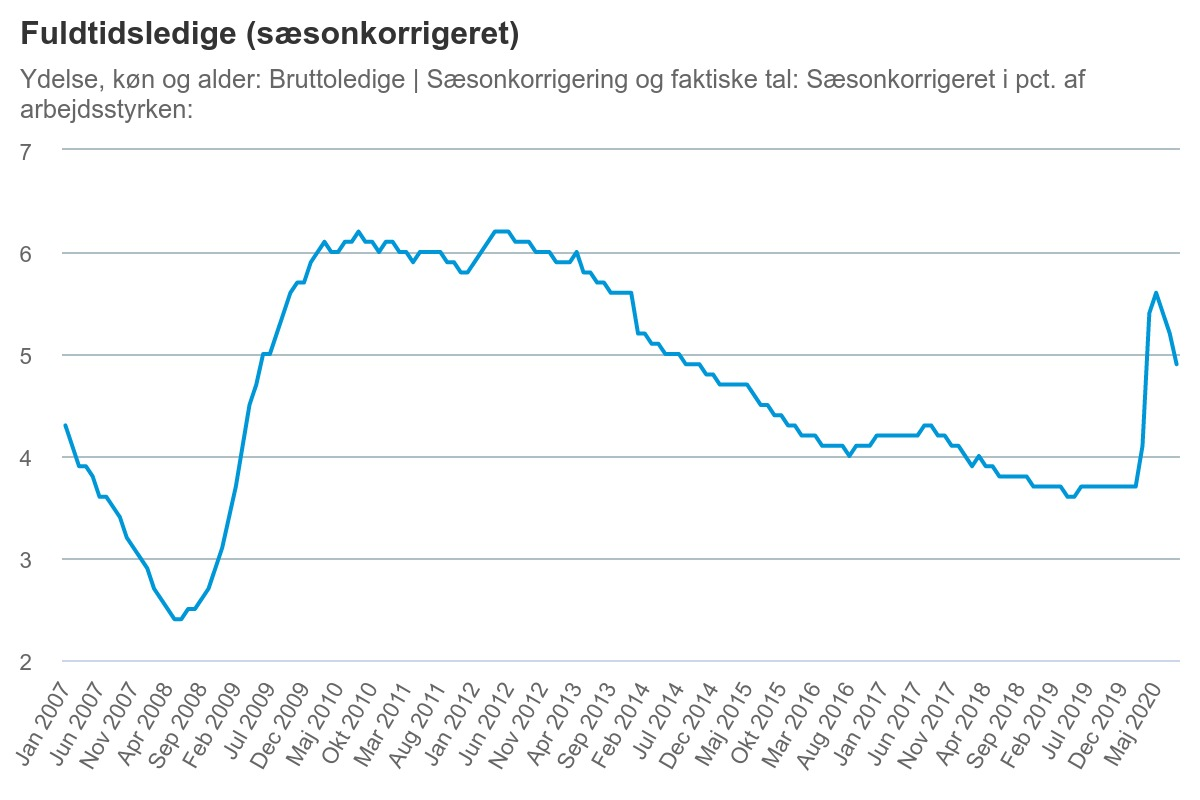
\includegraphics{figures/DK_unemployment_rate}%(dst.dk)

Figure ? displays the unemployment rate for the United States, the highest
populated western country -- four times that of the second highest -- with a
comparatively small public sector. Although the rate is generally higher than
that of Denmark it follows the same pattern, and again the number of people
looking for jobs is quite significant. The latest total number of unemployed
people in the U.S. is 12.6 million
%(https://www.bls.gov/news.release/empsit.nr0.htm).

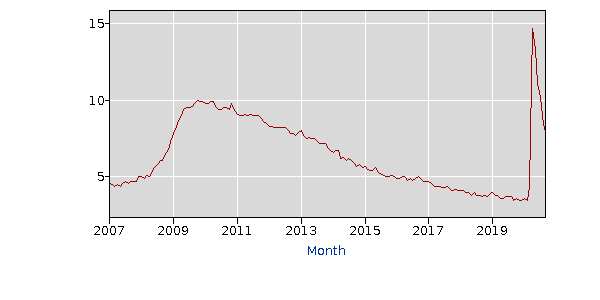
\includegraphics{figures/US_unemployment_rate}
%(https://data.bls.gov/timeseries/LNS14000000)

Besides the shear number of unemployed people, what is interesting is the ups
and downs of the economy. As mentioned generating better job applications faster
could arguably be most important on the back of an economic upturn. After the
2008 financial crisis, many of the jobs that were initially lost were recreated
and needed to be filled. Although the year 2020 is clearly considered an anomaly
(at least currently), this year serves to strengthen the point: in the U.S.
millions upon millions of people were fired only to be rehired months later. If
that process could somehow be streamlined, the gain could be quite significant.

\subsection{Getting a job}

\subsubsection{The numbers behind the process of getting a job}
How did people get their current job?
Lou Adler tried answering just this: He conducted an online survey
on linkedin based on 3000 answers, where in most of these answers
came from those actually hiring.

The results are outlined in the illustration underneath:
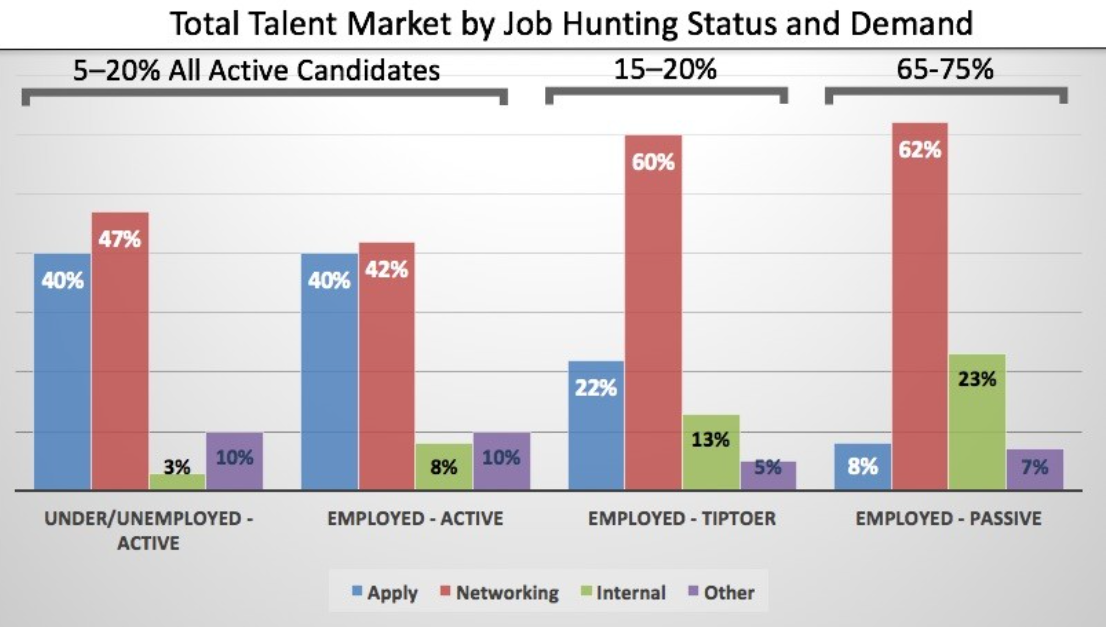
\includegraphics{figures/hiringpeople.png}
https://www.linkedin.com/pulse/new-survey-reveals-85-all-jobs-filled-via-networking-lou-adler/

Here we can see, that active candidates only represent 5-20 percent of the
entire jobmarket. Around 15-20 percent are only tiptoeing around the idea
of getting a new job, while the rest are passive candidates (meaning people who are
satisfied in their current position.).

Based on these graphs, we can see that at the very minimum, 42 percent of people are
hired based on networking, and that is only if you already have a job.
Whilst this percentage only goes up, the oppertunity for a job seeking person
to get hired based on an application goes down. This reflects the
most effective way to get hired is through internal applications or networking.
On the flip side, it also nicely illustrates just how stiff competition there actually is,
if your only way of getting hired is through sending applications.

When you send out an application, there is an 8.3 percent probability, that
they will actually invite you to a job interview. Furthermore it takes around
10-15 interviews, before one gets a job offer. Obviously it varies depending
on educational background, job type and many other factors, but this is the average.
Some quick math ( (((100/8,3)*10)+((100/8,3)*15))/2 = 150..) tells us, that it will
take an average of 150 ish applications before one gets a job offer.
https://talent.works/2017/09/22/how-long-does-it-take-to-get-a-job-60-days-if-youre-in-hr-or-sales/

All these applications add up, before one can reap the reward. According to a
study conducted surveying 2000 Americans, by recruitment agency Randstad US
discovering the “art of the job hunt”, it takes an average of five
months from when the job search begins, until one actually lands
the job.
https://www.swnsdigital.com/2018/10/it-takes-5-months-of-searching-to-land-a-job-study-finds/

To add insult to injurry, after all the hard work of creating an application, it can
take quite some time before the hiring managers actually respond, that is if they ever
bother answering your application to begin with.
It takes around 3 days between they receive the application, before they answer.
This is the case for the most in demand roles in society, for the less in demand roles
such as writers, nurses and unskilled labour, it can be anywhere from 10 to over 30 days.
https://talent.works/2017/09/22/how-long-does-it-take-to-get-a-job-60-days-if-youre-in-hr-or-sales/
On average one can expect to hear back from employers within a week 41 percent
of the time. Within a couple of weeks 85 percent of the time.
https://www.indeed.com/career-advice/finding-a-job/how-long-should-you-wait-to-hear-back-about-a-job

Below some of the more popular jobs are illustrated as a function of interview
rate on the left and response delay on the left:
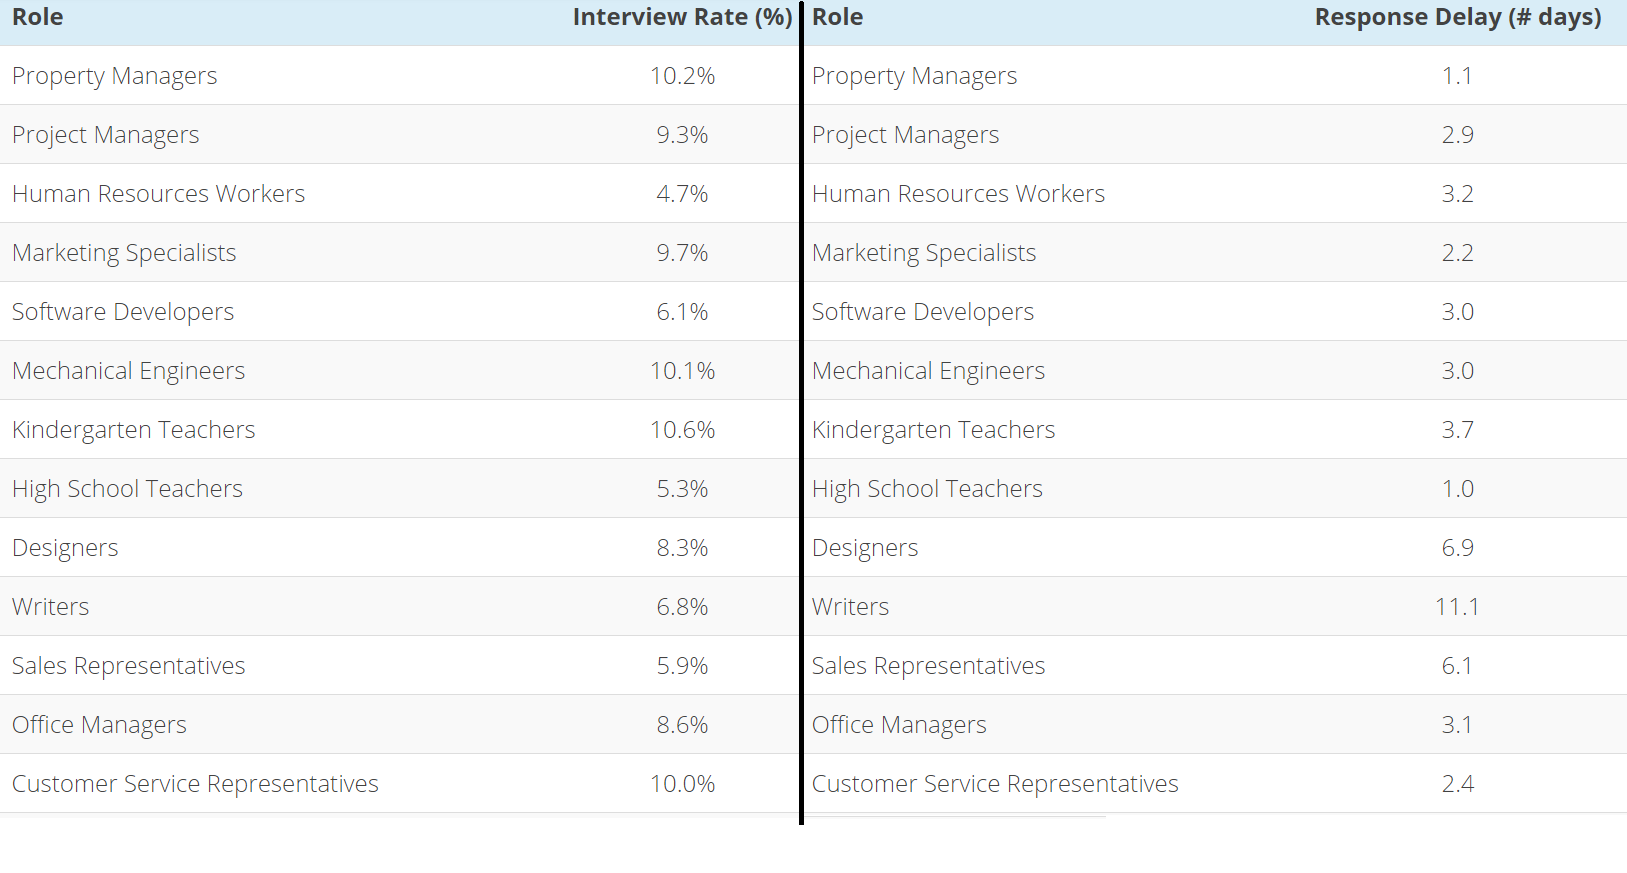
\includegraphics{figures/interviewratexdelay.png}
https://talent.works/2017/09/22/how-long-does-it-take-to-get-a-job-60-days-if-youre-in-hr-or-sales/
The interview rate is further supported from a danish online survey, that concluded
that 65 percent of people get an interview within the first 15 applications and
 82.5 percent of people get an interview within the first 30 applications.
 https://get2business.wordpress.com/2009/10/27/hvor-mange-ans%C3%B8gninger-skal-der-til-for-at-fa-et-job/

\subsubsection{Optimize ones interview rate}
There are many factors to consider, if one wishes to optimize ones
chances of getting an interview, one of the more empirical proven ones
is what time and day one sends their application.
To get the highest chances, you have to apply between early Tuesday morning
and Thursday before noon using the employers local time. Monday is even better,
increasing your chances by 46 percent in regard to the average.
If one should apply on another day, the most important factor is that
it's done before 10AM, since the interview chances drops below 5 percent for
the majority of late evening pplications.
https://insights.dice.com/2019/10/30/best-times-days-submit-resume/

One thing that is crucial, is how long ones resume is:
Having between 475-600 words is the optimal length, where the maxima is at
ca. 535 words. The optimal word count is illustrated below:
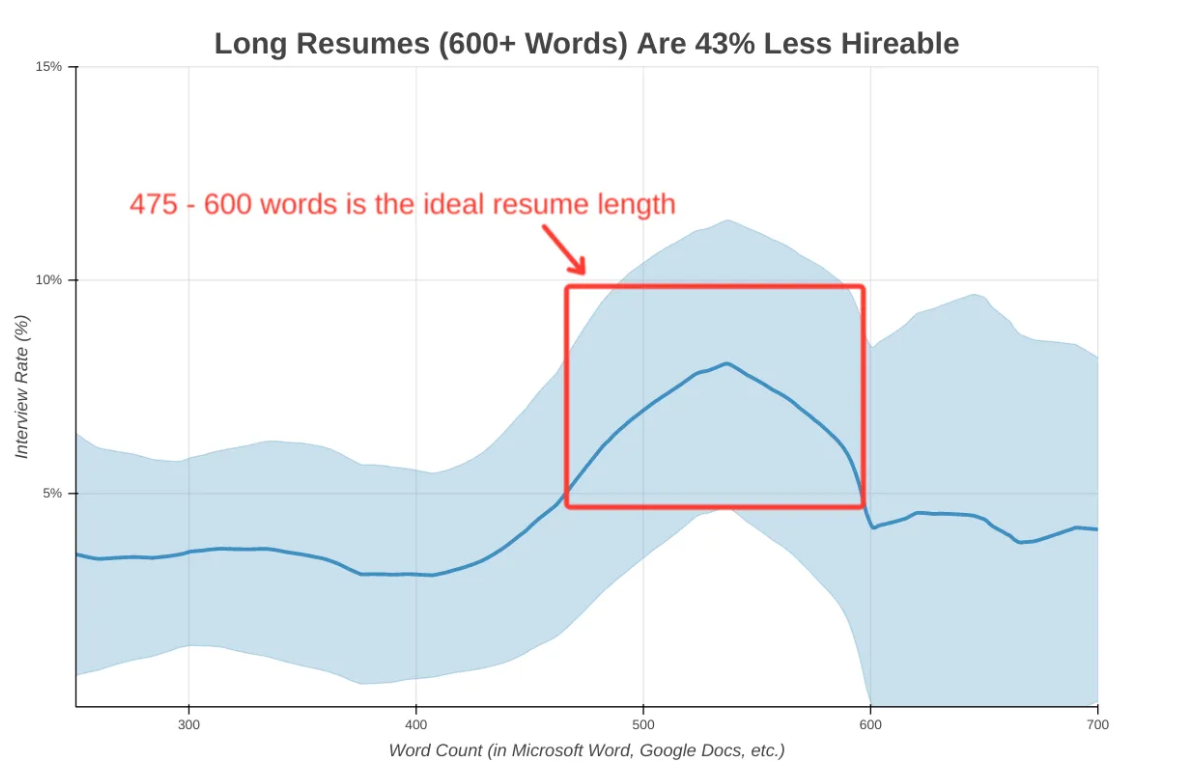
\includegraphics{figures/longresumegraph.png}
%https://talent.works/?utm_source=blog

Perhaps one of the most influential condition of weither you get an interview,
is how fast you are at applying:
Based on 30000 datapoints from the company Speedrecruiters, you need
to apply within the first 14 days to have a practical chance of getting an
interview. it is such that 50 percent of the people who got an interview
for the job applied within the first week, and 75 percent of those who
got an interview applied within the first 14 days, whilst the chancess of
getting an interview thereafter dwindles exponentially.
https://www.jobfinder.dk/artikel/her-bedste-tidspunkt-at-sende-din-ansoegning/220987

Other factors that influence the interview rate are as following:
1. Being a woman increases the chances by 48 percent.
2. Being older, but no older than 35, increases the interview rate by 25 percent.
3. Having more than one degree, increases ones chances by 22 percent.
4. Adding industry buzzwords increases your chances by 29 percent.
   e.g. If you are a software developer, then add buzzwords such as machine learning,
   artificial intelligence etc.
5. Demonstrating earlier job results using numbers increases chances by 40 percent.
   e.g. "Increased profits by 20 percent from Q3 to Q4"
6. Listing achievements, where you weren't in charge, but only a helping hand
 decreases your chances by 50 percent
   e.g. "Helped management organize financial reports" instead of "Organized financial reports"
7. Using leadership affiliated buzzwords increases your chances by 51 percent
8. Not using personal pronouns in the employment section increases your
chances by 55 percent.
9. Including a key skills section and buzzwords of the key skills increases your
 chances by 59 percent
10. Start ones sentences with distinct action verbs, increases ones chances by 140 percent.
   e.g. Do "Developed a mainframe architecture that drammatically increased efficiency"
   instead of "After surveying people, the mainframe architecture that increases efficiency was
   developed by me"
talent.works/2018/01/08/the-science-of-the-job-search-part-i-13-data-backed-ways-to-win/


%how long does it take to actually get a job

%how do these people then end up getting the job

%for the people sending applications, how many did they sen? ++ details

%best time to send applications, and why it can benefit people who
%dont have time there ++ howl ong should you wait with a followup

\subsection{Different expectations in a company}
Often companies have different expectations for structures and information's about the CV, so it will be relevant for the application.
Most of the time the companies expectations can be related to work experience and education,
and a CV could either be long or short depends on which company the person is writing to. Some people can write a long CV,
but it isn't necessarily a good CV, and people can write a short one but it isn't good enough.
Both of these statements could have some information that are not relevant to the company's requirement. Still there are some other
factors that can be included, and some companies would love to know what the person did in that particular year.
In that particular situation would be different from company to company, since those people who are working with humanities
can have human related criteria for getting a job in this area. The same goes for IT where they have more work with a computer
than any other people, because these jobs immerse themselves everyday with it. According to Computerworld it-jobbank,
they have actually examined a total of 6700 job posting in the year of 2015 and 2019 where the company was sorting all categories
that are related to IT, and they have published the top 10. It is shown between those years that the job-advertisements
have more of a technical, structured and professional knowledgeable side than before.
https://www.it-jobbank.dk/om-jobsoegning/karrierecenter/viden-om/it-karriere/disse-10-personlige-kompetencer-efterspoerger-virksomhederne?audiencetagid=140
That is tough very common, since will take good technical skills to do a very good job with the programming,
and structured can be a very important factor to have a good overview of a program,
and even if a new person with almost zero experience had to look at that,
it would still be possible to read trough the comments and understand it's functions. Below is the full result
of the 6700 job-advertisements that has been thoroughly examinant.

Top 10 in 2019 \\

Technical \\
Structured \\
Professional knowledge \\
Strong \\
Dynamic \\
Analytical \\
Responsible \\
Outgoing \\
Curious \\
Professional \\

Top 10 in 2015 \\

Structured \\
Technical \\
Dynamic \\
Strong \\
Informal \\
Responsible \\
Professional \\
Outgoing \\
Analytical \\
Committed \\

Research have also revealed that the most popular sentence for writing a CV can get it easier to get a job in IT-companies
Very popular to write:\\

Good for creating an overview and structure \\
Good for creating dialogue\\
Good at articulating you in writing and orally \\
Good at prioritizing your tasks \\
Good at seeing connections \\

Not very popular to write: \\

Good to collaborate and share your experiences \\
Good for keeping a cool head \\
Good at sharing your knowledge \\
Good at innovating, challenging and finding untraditional solutions \\
Good at uncovering and understanding customer needs \\
https://www.it-jobbank.dk/om-jobsoegning/karrierecenter/viden-om/it-karriere/disse-10-personlige-kompetencer-efterspoerger-virksomhederne?audiencetagid=140

In the situation of the contents and the document setup, there can be often of those different kind of setups,
there is one in particular and they are a comparative effectiveness research, and it's called
Patient-Centered Outcomes Research Institute (PCORI).
This organization have a purpose to fund research, so they can afterwords help patients and in the end try to make them better
informed to look at their health that they face every day.
https://www.pcori.org/about-us
They have a list to guide applicants who wants to work in the American Medical Association (AMA),
and this is only one of the examples of a requirement for a company.
In the situation of the contents and the document setup, there can be often of those different kind of setups,
there is one in particular and they are a comparative effectiveness research, and it's called
Patient-Centered Outcomes Research Institute (PCORI).
It's to determine which work best for which patients and which pose the greatest benefits and harms. %Redigere dette
They have a list to guide applicants who are want specifically work here: \\

Header: Include the Principal Investigator’s (PI’s) full name in the top left corner of the page header on every page. \\
Margins: Use at least half-inch margins. The header may fall within the top margin, but the body text should not begin closer than one half-inch from the edge of the page.
Font: Use size 11 Calibri for the main body of the text. Figures, tables and captions may be size 8 font.
Page Numbering: Each page must be numbered consecutively for each PDF upload. Each section of an uploaded document must begin with page 1.
Spacing: Use single spacing.
Document Format: Upload all attachments in PDF format. \\
https://help.pcori.org/hc/en-us/articles/213718977-What-are-the-page-formatting-requirements-for-submitting-an-application-

Even tough that applicants have wrote a good CV and they have used some good words to describe themselves,
there is a chance where keywords come in as a very important factor. In the digital world where often people have to send applications online, and over 90 %%
of all resumes and relevant information are being screened through an "Applicant Tracking System" (ATS). ATS is a scanning software system
that is designed to scan a resume for "work experience, skills, education, and other relevant information." https://www.zipjob.com/blog/ats-resume-test/
If it determines the resume is a good match for the position, it gets sent forward to the hiring manager.
Every time the ATS will do test, and it will determine if the test is a passing grade or it will be delete, so it will not even reach out to the hiring manager.
According to Caitlin Proctor it is stated that "Nearly 75 %%
of resumes are rejected because they’re not correctly formatted or keyword optimized." and there can be a lot of criteria
to get to the job you want. https://www.zipjob.com/blog/ats-resume-test/
So ind the end, the ATS is checking especially on five different elements when writing a resume, and that can be:
% Skal jeg beskrive om de 3 andre emner?
Standard formatting \\
Keyword optimization \\
Send as a Word document \\
Spell out abbreviations \\
Include relevant information \\
https://www.zipjob.com/blog/ats-resume-test/

\subsection{Required and situational content of a CV}
A CV  is “a short account of one’s career of qualifications prepared typically by an applicant for a position”1.
When applying for a position within a firm some aspects of a CV are required.
These requirements can come from the position or firm the CV is intended or from the definition of the CV itself.
Putting aside the firm or positions requirements, all CV’s must include the five following requirements to be defined as a CV:
1https://www.thebalancecareers.com/cv-vs-resume-2058495
1. Contact information
2. CV objective
3. Relevant skills
4. Work experience
5. Education
2https://novoresume.com/career-blog/how-to-write-a-cv
The substance of each requirement varies from applicant to applicant. However, every CV must include these five requirements to be effective.
A further explanation of each requirement is due:
Contact information is required as the firm at the bare minimum must have some way to contact you should you be accepted for the position.
CV objective is required as it specifies what and who the CV is intended and without it the CV can fill no purpose.
Relevant skills are required as without it you have no relation to the CV objective.
Work experience and Education is required as without it one has no qualifications.
as a CV is an account of one’s qualifications it is also possible to leave Eduaction and Work experience empty if one has none.
However it is then hardly an effective CV.3
Along with the requirements of CV there are also aspects which are situational.
These vary and must likely the firm or position in which one is applying to will lay out these aspects, or it is apparent from the position itself.
If not specified it is difficult to know what to include. To little and one will under-qualified, to much and the CV will be to long4, excesses and unorganised.
Therefore, it is essential to distinguish one’s CV with the right quantity and quality of situational content.
Lets examine some of the more typical situational content that could be included in a CV:
3https://www.thebalancecareers.com/cv-vs-resume-2058495#what-to-include-in-your-curriculum-vitae
4https://talent.works/?utm_source=blog
1. Proffesional association
2. Volunteer experience
3. Languages
4. Additional training courses
5. Publication
6. Awards/Honors
7. References
5https://zety.com/blog/what-to-include-in-a-cv
The effectiveness of a CV can drastically change due to use of situational content.
Therefore it is necessary to further explain each situational content:
Proffesional association is any trade unions, learned societies, regulatory univeristies and other inter-proffesional societies.
Many associations have certain prestiges and hold there member to a certain standard of quality.
Therefore a proffesional association can improve a CV if relevant.67
Volunteer experience is any voluunteer work relevant to the position.
Languages is any spoken or written language relevant to the position.
As most firms in our interconnected market interact with some multilingualism, languages can easily increase the quality of a CV.
Additional training courses are any extra courses relevant to the position.
Publication are any reports, books or other published materials that could show qualifications for the given position.
Awards and honors are any university or proffesional awards or honors given that show qualification for thr given position.
References are very situational, as putting references in a CV may make you seem unsure of yourself and in need of validation from others to show qualifications.
However, if a CV has the right references it can show assure employers of your qualifications and past experience.
6https://jobstars.com/professional-associations-organizations/
7https://money.usnews.com/careers/company-culture/articles/2018-09-05/the-perks-of-professional-organizations
